\section{Turbopompa}
\label{sec:turbopompa}

\subsection{Pompa}
\label{subsec:pompa}

....
\subsection{Turbina}
\label{subsec:turbina}

\subsubsection{Descrizione turbina}

\rfig{turbina_general}{Turbina ad impulso VC dell'F-1}{turbina_general}{0.45}

La turbina che fornisce la potenza necessaria alle pompe del sistema motore F-1 è definita come turbina a impulso (variazione di pressione statica solamente negli statori), e cosiddetta 2 row - velocity compounded (VC). Ovvero costituita da 2 file di rotori intramezzati da uno statore. Il gas caldo prima di passare in questa zona viene espanso in una schiera di ugelli che aumentano notevolmente la velocità: per le turbina VC, idealmente, tutta l'espansione avviene in questa zona. Successivamente i rotori, venendo impattati da un gas, sottraggono quantità di moto al fluido. Lo statore intermedio ha la funzione di reinidirizzare il flusso all'ingresso dell'ultimo rotore. Oltre a queste zone citate, nella turbina c'è una zona di ingresso, manifold, che convoglia il flusso ai nozzles. I nozzles, che sono generalmente convergenti-divergenti per una turbina VC, espandono il gas e lo incurvano per affrontare il primo rotore. Entrambe le i rotori della turbina sono costituiti da dischi i quali presentano dei 'fir tree' slot lungo la circonferenza, dove vengono inserite e rivettate le palette. Il rotore iniziale è calettato direttamente sull'albero, l'ultimo viene imbullonato sul primo e vengono separati da un distanziale. Le guarnizioni sono di diverso tipo, in questa sede non verranno approfondite, ma hanno il compito di contenere le perdite e quindi migliorare l'efficienza. 

\subsubsection{Dimensionamento turbina - scelte progettuali}

Il sistema turbina di un endoreattore ha una vita breve ma è sottoposto a parecchi carichi critici. Il design deve essere compatto e leggero, il fluido che espande deve avere un alto contenuto energetico, il lavoro specifico in uscita deve essere alto. La progettazione dell'elemento turbina è direttamente collegato al tipo di ciclo di alimentazione del motore, nel caso di un GG si vuole massimizzare il salto di pressione per minimizzare la portata spillata prima della camera di spinta (questo infatti massimizza l'impulso specifico del sistema). 

Per l'analisi del percorso aerotermodinamico del gas si tratta un flusso di gas combusti a chimica congelata (FE). Tali parametri fisici sono stati interpolati tramite MATLAB da una tabella fornita dal libro [] (Modern engieering for LRE systems, AIAA, Huzel, ...), dati ricavati da test sperimentali di NASA. Di seguito vediamo quali parametri principali vengono utilizzati per la scelta e il dimensionamento della turbina. 

\begin{itemize}

\item
\textbf{Spouting velocity:} è la velocità teorica che il flusso di gas avrebbe se espandesse dalla pressione di ristagno alla pressione di uscita (data dal rapporto $\epsilon$ di espansione)
\begin{empheq}{gather*}
C_0 = \sqrt{2C_{p,gg}T_{in} \left(1 - \epsilon^\frac{1-\gamma }{\gamma}\right)}
\end{empheq}

\item
\textbf{Rapporto isoentropico delle velocità:} è il rapporto tra velocità tangenziale del disco rotorico e la spouting velocity.

\begin{empheq}{equation*}
\frac{U}{C_0} = 
\end{empheq}

\parbox[t]{\dimexpr\textwidth-\leftmargin}{%

\begin{wrapfigure}{r}{0.4\linewidth}
	\centering
	\vspace{-\baselineskip}
	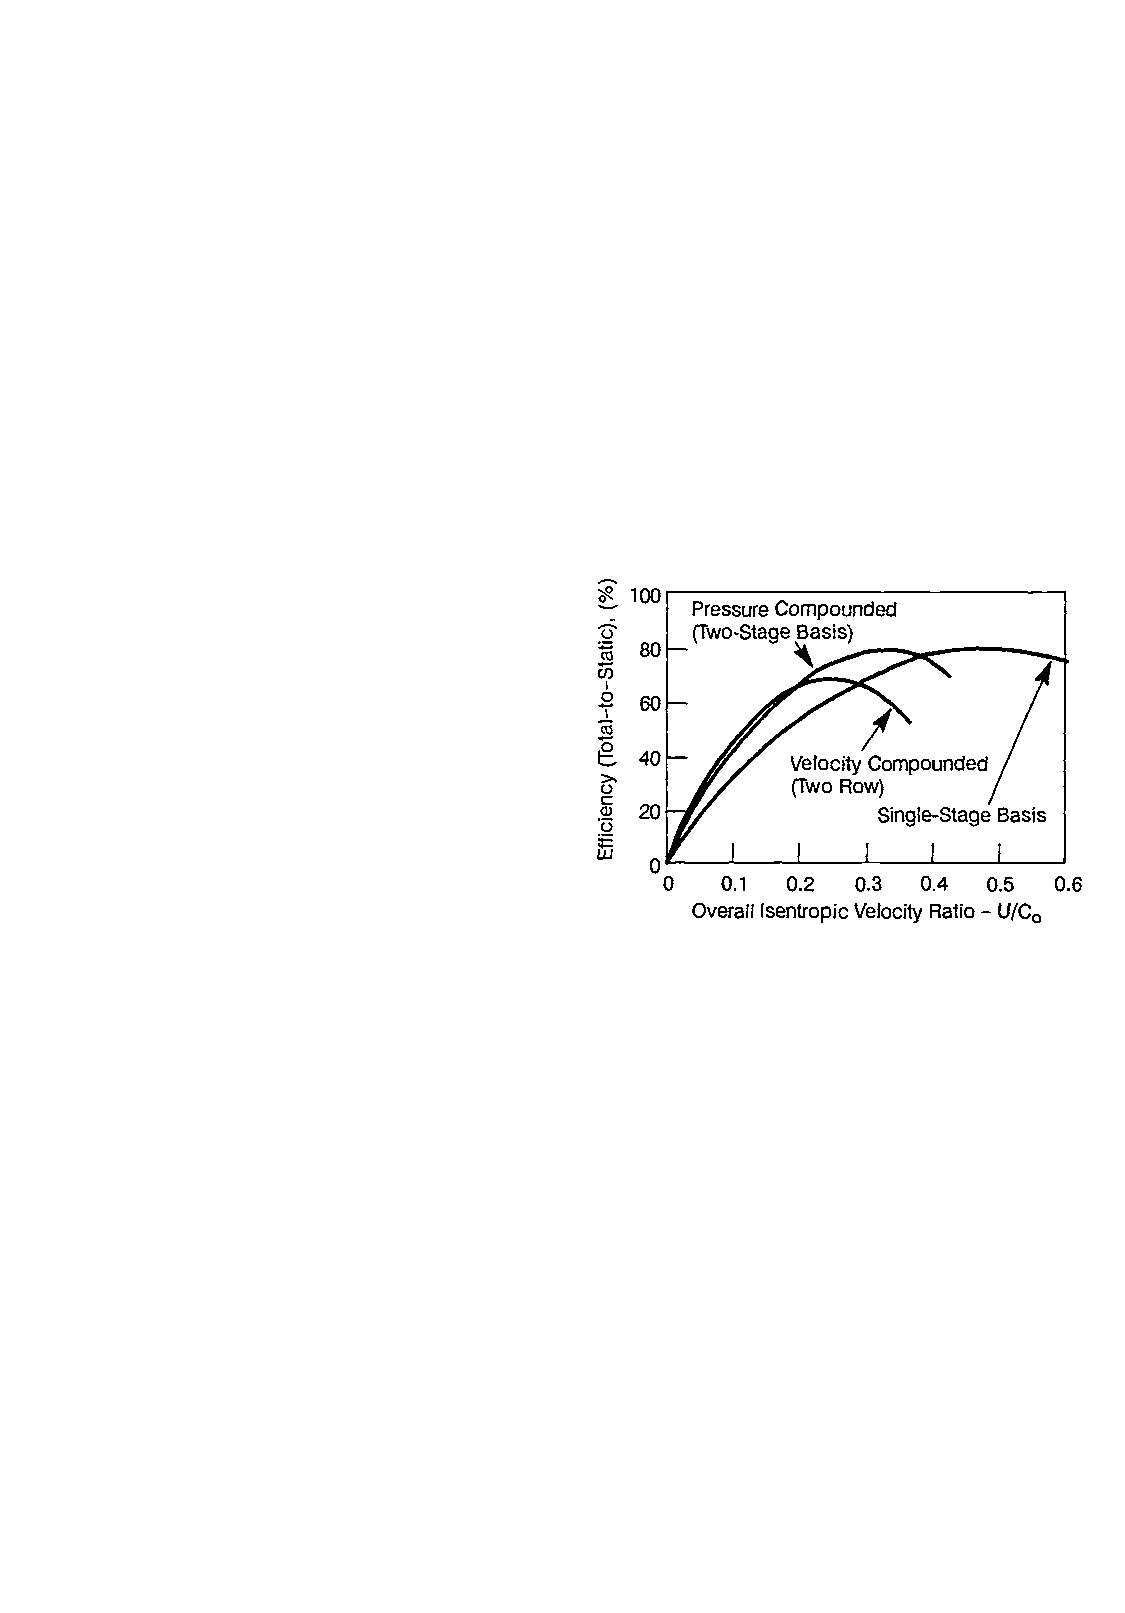
\includegraphics[width=\linewidth]{rendimenti_turbina}
	\caption{Rendimenti in funzione del rapporto di velocità}
	\label{fig:rendimenti_turbina}
\end{wrapfigure}

Questo valore è utile per capire la scelta progettuale effettuata per il tipo di turbina. Infatti, come già detto, nei cicli GG il salto di pressione in turbina è molto alto: questo implica un valore di $C_0$ elevato. Per avere una buona efficienza si possono percorrere più scelte progettuali (basandosi sul grafico x dei rendimenti). Si può scegliere di avere un alto rapporto di velocità con una singola ruota che 'assorba' tutta l'energia del flusso. Questo provocherebbe nel nostro caso una velocità di rotazione troppo elevata (quindi ingombro maggiore, inoltre la velocità di rotazione è fissata dalla pompa). Per usare altre turbine, cercando di avere un'alta efficienza si cerca di diminuire il rapporto di velocità aumentando gli stadi, ovvero la velocità del flusso è assorbita da più dischi che ruotano a velocità minori e sono più piccoli. Le turbine PC (generano il salto di pressione in tutti gli statori) sono più efficienti ma più pesanti. Per cui si è optato per un sistema VC, che ha buona efficienza a bassi rapporti di velocità e permette un risparmio in peso.
}

\end{itemize}